
\renewcommand{\thechapter}{4}
\chapter{Denoising Theory}

As has been discussed, the performance of double-beta experiments like EXO-200 is partially determined by their energy resolution.  In EXO-200, the energy resolution is limited by the scintillation energy resolution, which in turn is dominated by electronic noise in the APDs.  Significant effort must therefore be expended to understand and reduce the noise in the scintillation signals.

\begin{figure}
\begin{center}
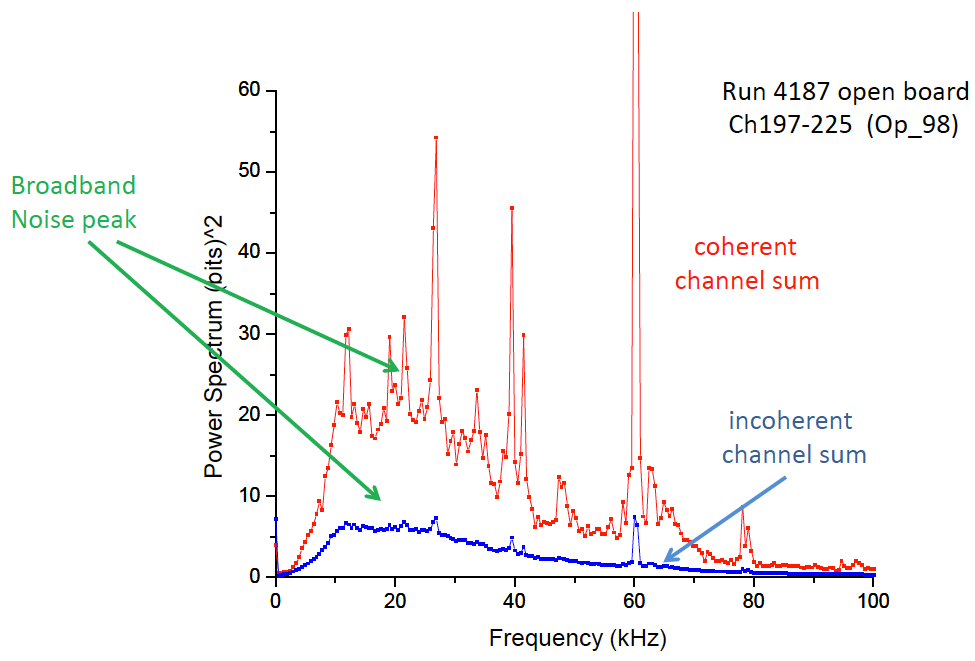
\includegraphics[keepaspectratio=true,width=\textwidth]{APDNoisePowerSpectrum.png}
\end{center}
\renewcommand{\baselinestretch}{1}
\small\normalsize
\begin{quote}
\caption{Coherent and incoherent noise power spectra for a sample set of APD channels without signal shaping.~\cite{ElectronicsUpgradeReport}}
\label{fig:APDNoisePowerSpectrum}
\end{quote}
\end{figure}
\renewcommand{\baselinestretch}{2}
\small\normalsize

When the noise in the APDs is studied, it was found that the individual APD channels met targetted root-mean-square noise levels of 2000 electrons.  However, rather than observing the noise on summed APD channels increase proportionally to the square root of the number of channels, the summed APD noise is roughly two to three times higher than projected.  This worse-than-expected scaling of the noise with channels indicates that noise across different channels is correlated, and further analysis confirms that the bulk of the noise on an unshaped APD waveform is correlated with other channels, as shown in Figure~\ref{fig:APDNoisePowerSpectrum}.  There are many possible sources of coherent noise in the hardware, and reducing the amount of coherent noise is a topic for further research.~\cite{ElectronicsUpgradeReport}

However, the observation that coherent noise is the dominant source of noise in the APDs, and thus also the limiting factor in EXO-200's energy resolution, means that it should be possible to exploit these correlations and reduce the level of noise in offline analysis.  This chapter will describe a scheme to accomplish that goal and produce an optimal estimate of scintillation energy which takes noise correlations into account.

It is worth noting that in fact there are a number of different qualitative approaches to reducing the noise levels in the scintillation channel.  In casual terms, we will refer to "passive" approaches as those in which components of our signals are weighted more or less heavily based on their relative signal-to-noise content.  "Active" approaches, by contrast, will be classified as those which attempt to improve the signal-to-noise content of signal components.  We have identified the following three types of denoising:
\begin{description}
\item[Frequency weighting] \hfill \\
On a given channel signal, weight more heavily the frequency components which contain larger signal-to-noise ratio.  This passive denoising scheme requires knowledge of the shapes in fourier space of a signal and the power spectrum of the noise.

\item[Channel weighting] \hfill \\
Different channels may have different levels of noise, so some may generally have higher-quality signals.  More importantly, though, the amount of signal on a given channel depends strongly on the proximity of the APD gang to the source of scintillation within the detector.  This passive denoising scheme therefore allows us to weight more heavily the channels which have more scintillation, provided we can identify these weights on an event-by-event basis.  This requires knowledge of the magnitude of noise on each channel and of the correspondence between event position and signal magnitude on each APD gang; the latter is described by the lightmap, described earlier.

\item[Noise subtraction] \hfill \\
This active form of denoising consists of using correlations between noise on different channels to produce a better estimate of the noise component of signals than each signal taken independently could provide.  To accomplish this, we will require detailed information about the pairwise noise correlations across channels at each frequency.
\end{description}

In the following, we will describe a general linear operator on the APD signals which in principle can accomplish each of these forms of denoising, and we will presume that all of the described inputs are available; by identifying the parameters for that linear operator which are optimal, we can be confident that the denoising operator we produce will accomplish all three forms of denoising described above.

\section{Setup}

We first establish a number of notational conventions:
\begin{itemize}
\item $i$, $j$ will represent indices over APD channels.
\item $t$ will represent the time indices of a discrete waveform.
\item $f$, $g$ will represent the frequency indices of Fourier-transformed waveforms.
\item $a$, $b$ will represent indices of signals in an event.
\item For a waveform $*[t]$, we will represent the discrete Fourier transform of that waveform with $\widetilde{*}[f]$, where the particular convention used to evaluate the Fourier transform is not significant.
\item For a Fourier-transformed waveform $\widetilde{*}[f]$, we denote the real and imaginary parts of that waveform by $\widetilde{*}^R[f]$ and $\widetilde{*}^I[f]$, respectively.
\end{itemize}

We describe the data as a collection of discretely sampled waveforms, $X_i[t]$.  We assume that all signal times and shapes are already known, so we can model the waveforms by $X_i[t] = \sum_a M_{ia}Y_{ia}[t] + N_i[t] + b_i$, where $Y$ is the shape of signal $a$ on channel $i$, $M$ is the magnitude of that signal, and $N$ and $b$ represent the electronic noise and baseline, respectively, of the channel.

\begin{figure}
\begin{center}
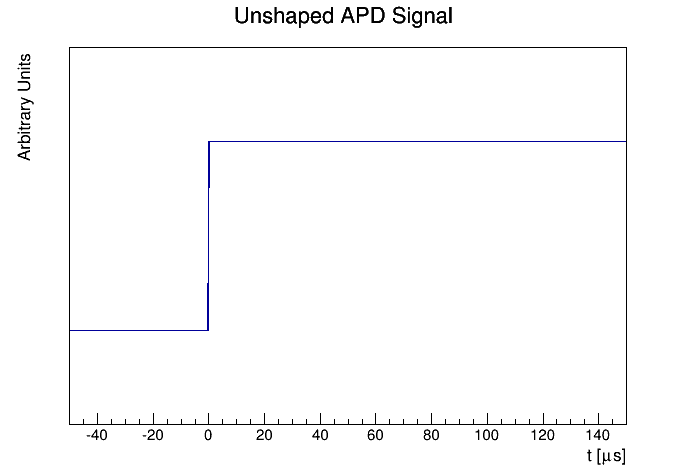
\includegraphics[keepaspectratio=true,width=\textwidth]{scripts/UnshapedAPDWaveform.png}
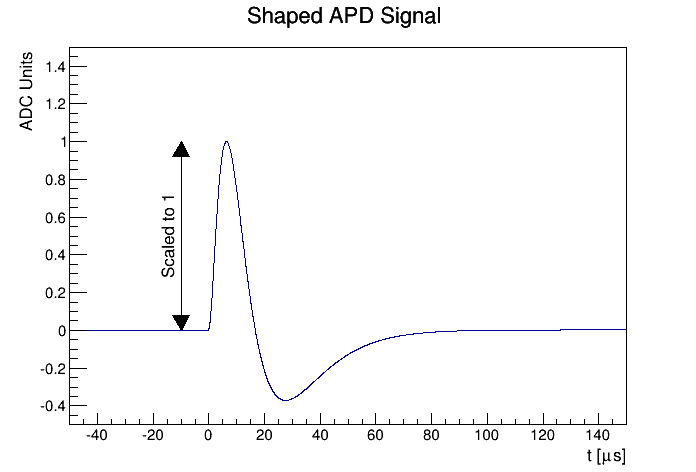
\includegraphics[keepaspectratio=true,width=\textwidth]{scripts/ShapedAPDWaveform.png}
\end{center}
\renewcommand{\baselinestretch}{1}
\small\normalsize
\begin{quote}
\caption{Shaped and unshaped APD waveforms.  The normalization is shown to make the peak of the shaped waveform have a magnitude of one, and the time axis is shifted so that the unshaped waveform is a step function centered at $t=0$.}
\label{fig:SampleAPDTemplates}
\end{quote}
\end{figure}
\renewcommand{\baselinestretch}{2}
\small\normalsize

To break the degeneracy between $M$ and $Y$, we choose to fix the magnitude of the template signal $Y$.  We choose to require that the signal $Y$ has its peak at one when its baseline lies at zero, as illustrated in figure~\ref{fig:SampleAPDTemplates}.  (Note that the baseline here is not the same as the zero-frequency component; rather, this asserts that $Y$ goes to zero for times far away from the time of the signal.)

Noise correlations will be much simpler in frequency space, so we take the Fourier transform and drop the zero-frequency component to obtain \[\widetilde{X}_i[f] = \sum_a C_{a}\widetilde{Y}_{ia}[f] + \widetilde{N}_i[f].\]

\subsection{The Noise Model}

We will assume that there are two sources of noise in this model.  First, the electronic noise $N_i[t]$ is assumed to be random.  We require that noise with different frequencies is uncorrelated:
\[\left< \widetilde{N}_i[f] \widetilde{N}_j[g] \right> = 0 \text{~when~} f \ne g.\]
The noise correlations $\left< \widetilde{N}_i[f] \widetilde{N}_j[f] \right>$ are assumed to be known; our means for measuring them are described [ELSEWHERE].

The second random variable will be the magnitude of the signal itself, $C_s$.  When an energetic decay occurs in bulk of the detector, it will release some number of photons and electons which reflects the energy of the decay; however, the number of photons and electrons actually collected by sensors is randomly distributed.  We now consider the sources of that randomness.

On the wire channels, all charge is directed by the electric field to deposit in a single location; so the dominant source of randomness comes from impurities.  Electrons are absorbed by impurities through their trajectory across the bulk of the Xenon; the expected quantity of charge decays exponentially in time with some half-life $T$.  We can describe the number of lost electrons by a Poisson process.  However, a typical deposit in out Q-value will produce tens of thousands of electrons, from which at most about $10\%$ may be lost to purity, making Poisson noise negligible in this situation.  Moreover, there is no available information in the charge channel which can reduce this source of noise; so it is proper to associate this source of uncertainty as a part of the irreducible detector resolution in the charge channel, and we will not treat it further.

On the APD channels, we detect photons which travel from the source of the energy deposit to the face of the APD.  The paths of optical photons, and their reflection off of detector surfaces, is highly variable, so it is reasonable to model the number of photons depositing on any particular APD as Poisson-distributed.  A typical deposit in our Q-value may deposit $10-100$ photons on each APD, depending strongly on the location of the deposit; we find that on a single APD channel Poisson noise is very important.  Suppose that for a deposit of energy $E$, we expect an average of $Q_{tot}$ photons to be produced and $Q_k$ photons to deposit on APD channel $k$.  Then the number of photons $P_k$ deposited on APD channel $k$ will follow a multinomial distribution with the properties:
\begin{itemize}
\item $\left< P_k \right> = Q_k$
\item $\left< P_k P_{\ell} \right> = Q_k Q_{\ell} \left( 1 + \delta_{k\ell}Q_k^{-1/2}Q_{\ell}^{-1/2} - Q_{tot}^{-1}\right)$
%If k = ell,
%Variance = <(P_k - Q_k)^2> = <P_k^2> - 2Q_k^2 + Q_k^2 = <P_k^2> - Q_k^2
%but variance = Q_tot * Q_k/Q_tot * (1-Q_k/Q_tot)
%So, <P_k^2> = Q_k^2 + Q_k*(1-Q_k/Q_tot)
%            = Q_k^2(1 + 1/Q_k - 1/Q_tot)
%Otherwise,
%Covariance = <(P_k - Q_k)(P_l - Q_l)> = <P_k P_l> - Q_kQ_l
%But covariance = -Q_k*Q_l/Q_tot
%So <P_k P_l> = Q_k Q_l (1-1/Q_tot)
\end{itemize}

Note that this implies that to fully understand the noise on our APDs, we must have some a priori estimate of $Q_tot$; this requires us to have an a priori estimate of the deposit energy.  It will be important to ensure our estimator does not bias us toward whatever estimate is provided; we will return to this point.

Our noise model, as we have said, is \[\widetilde{X}_i[f] = \sum_s C_s\widetilde{Y}_{is}[f] + \widetilde{N}_i[f].\]  But it will be advantageous to fix the normalization of $\widetilde{Y}$ to something consistent.  In the case of wires, we use the usual normalization encountered in reconstruction: a deposit waveform should be normalized so that its peak lies $1$ ADC above the baseline.  Furthermore, in our model we must characterize the expected signal on every waveform from a given deposit; to generate the expected induced signals on neighboring wires, we use the same digitizer used in Monte Carlo, and scale by the same factor used on the deposit channel.

On APDs, there is no advantaged channel which should be used to set a scale, as we did for wires.  However, there is a preferred energy scale: the lightmap we use is generated from photopeak events at the Thallium-208 gamma line at $2615$ keV, and this normalization is preserved in the lightmap file format.  So, the lightmap explicitly records the signal size (in ADC counts from baseline to peak) expected from a $2615$ keV gamma-like deposit at all positions and times, and we can preserve that normalization here.  APD-channel $\widetilde{Y}_{is}$ are therefore normalized to the number of ADC counts expected from a $2615$ keV deposit, and $C_{is}$ indicates the measured energy of the deposit in units of $2615$ keV.

We can specify these factors explicitly.  Let $M_k(x,t)$ be the yield in ADC counts expected on APD channel $k$ from a single-site $2615$ keV deposit at position $x$ and time $t$.  Let $\widetilde{Y}_{\tau}[f]$ represent a $1$-ADC APD signal occurring at time $\tau$ within a waveform.  (We assume for now, as we do in the rest of the analysis, that the shaping times on all APDs are identical.)

Let $E_{exp}$ be the a priori expected energy of the deposit, in units of $2615$ keV; if we expect $c$ photons per $2615$ keV deposited, we then can use $Q_{tot} = c \cdot E_{exp}$.  We can also write $Q_{ks}$ in terms of $C_s$ if we have some conversion factor between ADC counts and incident photons on an APD channel $k$.  Let $g_{k}(t)$ be this gain factor, as a function of time; then \[\frac{Q_{ks}\cdot g_k(t)}{M_k(x,t)} = E_{exp} = \left<C_s\right>.\]

\subsection{Optimization and Constraints}

For each signal, we wish to identify a denoising operator which acts on the Fourier components of all of the waveforms and yields an estimate of the magnitude of that signal.  To make the problem tractable, we stipulate that this operator must be linear; so our estimate of the unknown parameter $C_s$ will be
\[ \widehat{C}_s = \sum_{if} A_{ifs} \widetilde{X}_i^R[f] + B_{ifs} \widetilde{X}_i^I[f]\]

For each event and each signal, the goal of denoising is to find a set of coefficients $A_{ifs}$, $B_{ifs}$ which minimizes the expected square-error in this quantity,
\[ \epsilon = \left< \left(C_s - \widehat{C}_s\right)^2\right> \]

It will turn out to be necessary, to make the problem tractable, to make the additional assumption that this denoising operator produce an unbiased estimate.  This is expressed by the constraint:
\[ \left< C_s - \widehat{C}_s\right> = 0 \]
Although this constraint is necessary for mathematical tractability, it is worth noting that it is not required by physics.  Releasing this constraint would permit biased estimators, but might permit the use of a narrower region of interest with better signal-to-background ratio.  For instance, it might permit a mono-energetic peak to appear with asymmetric tails.  A future project could involve releasing this constraint and checking whether the resulting resolution is improved; however, the increase in required computation makes this infeasible for us.

\section{Derivation}

We are now in a position to derive the optimal denoising estimator.  We start by expanding the square-error value:
\[
\begin{array}{rcl}
\epsilon &=& \left< \left(C_s - \widehat{C}_s\right)^2\right> \\

&=& \left<\left(C_s - \sum_{if} \left[A_{ifs} \widetilde{X}_i^R[f] + B_{ifs} \widetilde{X}_i^I[f]\right]\right)^2\right> \\

&=& \left<\left(C_s - \sum_{if} \left[A_{ifs}\widetilde{N}_i^R[f] + B_{ifs}\widetilde{N}_i^I[f]\right]
                    - \sum_{ifr}C_r\left[A_{ifs}\widetilde{Y}_{ir}^R[f] + B_{ifs}\widetilde{Y}_{ir}^I[f]\right]
    \right)^2\right>
\end{array}
\]
We assume that the electronic and Poisson noise terms are uncorrelated:
%\[
%\begin{IEEEeqnarray*}{rcll}
%\epsilon &=& \IEEEeqnarraymulticol{2}{l}{
%\left<\left(\sum_{if} \left[A_{ifs}\widetilde{N}_i^R[f] + B_{ifs}\widetilde{N}_i^I[f]\right]\right)^2\right> +
%             \left<\left(C_s - \sum_{ifr}C_r\left[A_{ifs}\widetilde{Y}_{ir}^R[f] + B_{ifs}\widetilde{Y}_{ir}^I%[f]\right]\right)^2\right>}\\
%
%&=& \left<\left(\sum_{if} \left[A_{ifs}\widetilde{N}_i^R[f] + B_{ifs}\widetilde{N}_i^I[f]\right]\right)^2\right> +
%     \left<\left(\sum_{ifr}C_r\left[A_{ifs}\widetilde{Y}_{ir}^R[f] + B_{ifs}\widetilde{Y}_{ir}^I[f]\right]\right)^2\right> -
%     2\left<C_s \sum_{ifr}C_r\left[A_{ifs}\widetilde{Y}_{ir}^R[f] + B_{ifs}\widetilde{Y}_{ir}^I[f]\right]\right> +
%     \left<C_s^2\right> \\



%&=& \sum{ijfg}\left[&A_{ifs}A_{jgs}\left<\widetilde{N}_i^R[f]\widetilde{N}_j^R[g]\right> + \\
%& &                 &A_{ifs}B_{jgs}\left<\widetilde{N}_i^R[f]\widetilde{N}_j^I[g]\right> + \\
%& &                 &B_{ifs}A_{jgs}\left<\widetilde{N}_i^I[f]\widetilde{N}_j^R[g]\right> + \\
%& &                 &B_{ifs}B_{jgs}\left<\widetilde{N}_i^I[f]\widetilde{N}_j^I[g]\right> \right] + \\
%& &


%\end{array}
%\]
% IEEEeqnarray would have the benefit of letting me merge across multiple columns, as used here.
% Problem: latex complains when I start a group like \left[ which trails across a line.


















\section{Preconditioning}

The matrix equation we wish to solve takes the form:
\[\begin{pmatrix}
E+P & L\\
L^\top & 0
\end{pmatrix}
X = 
\begin{pmatrix}
0 \\ I
\end{pmatrix}\]
Let us define $D = diag(E)$ and approximate
\[\begin{pmatrix}
E+P & L\\
L^\top & 0
\end{pmatrix}
\approx
\begin{pmatrix}
D & L\\
L^\top & 0
\end{pmatrix}\]
This approximate form is easy to invert, and can be used to precondition our problem for better numerical behavior.

We can further factor this approximate form of the matrix:
\[
\begin{array}{cccc}
\begin{pmatrix}
D & L\\
L^\top & 0
\end{pmatrix}
&=&
\begin{pmatrix}
D^{1/2} & 0\\
L^\top D^{-1/2} & -H^\top
\end{pmatrix}
&
\begin{pmatrix}
D^{1/2} & D^{-1/2}L\\
0 & H
\end{pmatrix}\\[1em]
&=&

\begin{pmatrix}
D^{1/2} & 0\\
0 & I
\end{pmatrix}
\begin{pmatrix}
I & 0\\
L^\top D^{-1/2} & -H^\top
\end{pmatrix}
&
\begin{pmatrix}
I & D^{-1/2}L\\
0 & H
\end{pmatrix}
\begin{pmatrix}
D^{1/2} & 0\\
0 & I
\end{pmatrix}

\end{array}
\]
where $H$ is defined uniquely by $H^\top H = L^\top D^{-1} L$.  (The solution is guaranteed to be real because D is positive-semidefinite -- it consists of noise variance terms, which are non-negative.)

The two diagonal factors are easily inverted; we further define
\[
\begin{array}{cc}
K_1 =
\begin{pmatrix}
I & 0\\
L^\top D^{-1/2} & -H^\top
\end{pmatrix}
&
K_1^{-1} =
\begin{pmatrix}
I & 0\\
{H^\top}^{-1}L^\top D^{-1/2} & -{H^\top}^{-1}
\end{pmatrix}\\
K_2 =
\begin{pmatrix}
I & D^{-1/2}L\\
0 & H
\end{pmatrix}
&
K_2^{-1} =
\begin{pmatrix}
I & -D^{-1/2}LH^{-1}\\
0 & H^{-1}
\end{pmatrix}
\end{array}
\]
and then follow the standard proscription for preconditioning a linear system:
\begin{gather*}
K_1^{-1} \begin{pmatrix}D^{-1/2}&0\\0&I\end{pmatrix}
\begin{pmatrix}
E+P & L\\
L^\top & 0
\end{pmatrix}
\begin{pmatrix}D^{-1/2}&0\\0&I\end{pmatrix} K_2^{-1} Z = 
K_1^{-1} \begin{pmatrix}D^{-1/2}&0\\0&I\end{pmatrix} \begin{pmatrix}0\\I\end{pmatrix}\\
Z = K_2 \begin{pmatrix}D^{1/2} & 0\\0 & I\end{pmatrix}X
\end{gather*}
which reduces to
\begin{gather*}
K_1^{-1} 
\left[
\begin{pmatrix}D^{-1/2}ED^{-1/2}&0\\0&0\end{pmatrix}
+
\begin{pmatrix}D^{-1/2}PD^{-1/2}&D^{-1/2}L\\L^\top D^{-1/2}&0\end{pmatrix}
\right]
K_2^{-1} Z = 
\begin{pmatrix}0\\-{H^\top}^{-1}\end{pmatrix}\\
X = \begin{pmatrix}D^{-1/2}&0\\0&I\end{pmatrix}K_2^{-1}Z
\end{gather*}

This preconditioned set of equations is numerically quite stable.  It is also possible to provide an excellent initial guess $Z_0$ by taking the approximate form of the matrix to be exact, yielding
\[
Z_0 = \begin{pmatrix}0\\-{H^\top}^{-1}\end{pmatrix}
\]
Based on these various advantages, it is this system which we attempt to solve rather than the original form.  Below we define matrices $A$ and $B$ for convenience, and summarize the system to be solved:
\[\begin{array}{rcl}
A &=& K_1^{-1} 
\left[
\begin{pmatrix}D^{-1/2}ED^{-1/2}&0\\0&0\end{pmatrix}
+
\begin{pmatrix}D^{-1/2}PD^{-1/2}&D^{-1/2}L\\L^\top D^{-1/2}&0\end{pmatrix}
\right]
K_2^{-1}\\
B &=& Z_0 = \begin{pmatrix}0\\-{H^\top}^{-1}\end{pmatrix}\\
AZ &=& B\\
X &=&  \begin{pmatrix}D^{-1/2}&0\\0&I\end{pmatrix}K_2^{-1}Z
\end{array}\]


\section{Solver}

The matrix $Z$ for which we attempt to solve will have as many columns as there are signals we wish to simultaneously refit within an event; in the case of light-only denoising and with the restriction that we only examine events with one scintillation signal, $Z$ will always have exactly one column.  In general, though, it may be desirable to denoise events with multiple scintillation signals; or it may be beneficial to denoise certain wire channels (which may include wire signals) simultaneously with the APD channels.  In these cases the number of columns may be larger -- five or six columns may not be unusual.  In such cases it would be possible to solve for each column of $Z$ independently, but more efficient to solve the entire system simultaneously.  In this way, information obtained from multiplying the matrix by one column may be exploited to solve the other columns as well, effectively multiplying the benefit from each matrix-multiplication by the number of columns of $Z$.\footnote{In practice the improvement is not quite so impressive, for two reasons: the vectors which are most useful toward solving one column may not be the most useful toward solving another; and some columns may achieve a solution earlier than others, yet are difficult to terminate without restarting the solver entirely.  These challenges have not appeared to be significant for this particular system.}

The algorithm which we have selected for solving this system is the block variant of the stabilized biconjugate-gradient method (Bl-BiCGSTAB) [CITE THIS].  It is reproduced here in the form used by our code.

\begin{algorithmic}
\STATE $R \gets B-AZ_0$
\STATE $P \gets R$
\STATE $\widetilde{R_0} \gets R$
\WHILE{any column of $R$ has a magnitude greater than desired}
  \STATE $V \gets AP$
  \STATE Solve $(\widetilde{R_0}^\top V)\alpha = (\widetilde{R_0}^\top R)$ for $\alpha$.
  \STATE $R \gets R - V\alpha$
  \STATE $T \gets AR$
  \STATE $\omega \gets {\langle T,S\rangle_F} / {\langle T,T\rangle_F} $
    \COMMENT{where $\langle\cdot,\cdot\rangle_F$ is the Frobenius matrix norm.}
  \STATE $Z \gets Z + P\alpha + \omega R$
  \STATE $R \gets R - \omega T$
  \STATE $R$ currently equals $B-AZ$; if it is small enough, terminate.
  \STATE Solve $(\widetilde{R_0}^\top V)\beta = -(\widetilde{R_0}^\top T)$ for $\beta$.
  \STATE $P \gets R + (P - \omega V) \beta$
\ENDWHILE

\end{algorithmic}

Since each column of $Z$ corresponds to one signal we are refitting, the norm of the corresponding column of $R$ tells us how well we have identified the optimal magnitude estimator for that signal; thus, to test for termination we should evaluate the norm of each column of $R$, and while any of those norms are above some threshold, the solver must be permitted to continue.  Because our resolution is only on the order of $1\%$, solutions generally need not be very accurate; in practice, we establish reasonable thresholds by plotting resolution against threshold for a small subset of data, and observing when the resolution stops improving.

\section{Implementation}

Although the previous section described the algorithm used for solving these matrix equations, in practice the processing time required is significant.  There are certain implementation tricks which can be applied with significant impact.  These are described here.

FILL-IN: Poisson multiplication using common factors.

After reducing the complexity of handling Poisson terms in this way, the handling of electronic noise terms in matrix multiplication becomes the computational bottleneck.  The structure of the problem is that the matrix containing electronic noise terms is block-diagonal; that is, it consists of one dense block per frequency component, with each block lying on the diagonal and where the number of rows and columns is twice the number of channels being denoised (except for the last frequency component, where imaginary terms are identically equal to zero).  The problem of handling electronic noise terms thus consists of $1024$ matrix-matrix multiplications, with the left matrix of approximate size $300\times300$ and the right matrix of approximate size $300\times O(1)$.\footnote{The number of columns in the right matrix is equal to the number of signals, which may be sometimes $3-5$ or more; however, it is always much smaller than $300$, and describing it as $O(1)$ captures this fact.}

The key points here which create an opportunity for optimization are that:
\begin{itemize}
\item The electronic noise terms generally do not change event-by-event.  They are treated as constant across many runs.
\item It is possible to multiply two $N \times N$ matrices together much faster than it is possible to perform $N$ multiplications of an $N \times N$ matrix with $N$ $N \times 1$ matrices.  This can be achieved with a combination of algorithms faster than naive $O(N^3)$ speed and exploitation of low-level computer hardware features such as the CPU cache. [Provide a citation!]
\end{itemize}
What we wish to do, then, is reorganize the solver algorithm so that whenever multiplication by the electronic noise matrix is required, rather than performing that multiplication on a ``skinny" $300 \times O(1)$ matrix, we pack together many such ``skinny" matrices into a single matrix with many columns.  Multiplication can then be performed in bulk; and individual columns from the result can be extracted and used as before.

Additionally, it is important that matrix multiplication be made as fast as possible.  It has long been known that matrix multiplication provides significant opportunities for low-level optimizations. For example, most of the time taken by naive matrix multiplication is spent fetching and writing data to and from RAM.  Significant speedups can be achieved by minimizing the number of CPU cache misses, which can be accomplished by operating on matrices in blocks with size chosen so they fit entirely in the cache.  Multiplication instructions can also often be packed into vector instructions such as SSE or AVX.  For extremely large matrices, there are even algorithms which require fewer than $O(N^3)$ multiplications, and these can sometimes be beneficial.

Optimization of matrix-matrix multiplication is a large field, but fortunately there are a number of well-tuned software libraries implementing matrix multiplication well-tuned to specific machines.  These libraries generally provide the standard Basic Linear Algebra Subroutines (BLAS) interface, making them interchangeable with ease.  In this instance, Intel's MKL library has been used; benefits to this implementation are its availability (MKL is installed on both the SLAC and NERSC computing systems.) and its adaptability (MKL will detect a machine's architecture at runtime, and select a well-tuned codepath then; this is in contrast to some other BLAS implementations which must be compiled on the particular machine where they will be used.).

Finally, implementation at NERSC has the interesting feature that NERSC's computing systems are designed for multi-core processing.  The Hopper and Edison computing systems at NERSC allocate whole nodes, each of which contains 24 cores.  Although it is possible to simply run 24 independent processes on each node, memory on NERSC machines is highly constrained; memory use can be reduced by sharing certain large data structures across multiple cores on a node.  Additionally, as more events are packed together for electronic-noise multiplication, greater savings can be realized; so it is better to handle many events in coordination.  To this purpose, a multi-threaded version of the program has been developed to exploit portions of the code which are conveniently distributed.  Because NERSC nodes have a Non-Uniform Memory Access (NUMA) architecture, processes are constrained to only run on cores with a similar memory access pattern; on Hopper this results in four 6-threaded processes per node, while on Edison this results in two 12-threaded processes per node.


Outline new algorithm demonstrating multi-threading and batch handling.

\begin{algorithmic}
\STATE $E$ is a list of events.
\WHILE{there are events to read}
  \STATE Push the next event $E_i$ onto $E$.
  \STATE Compute $A_i$ and $Z_0^i$, the matrix and initial guess for event $E_i$.
  \STATE $R_i \gets B-A_i Z_0^i$
  \STATE $P_i \gets R_i$
\ENDWHILE

\STATE $R \gets B-AZ_0$
\STATE $P \gets R$
\STATE $\widetilde{R_0} \gets R$
\WHILE{any column of $R$ has a magnitude greater than desired}
  \STATE $V \gets AP$
  \STATE Solve $(\widetilde{R_0}^\top V)\alpha = (\widetilde{R_0}^\top R)$ for $\alpha$.
  \STATE $R \gets R - V\alpha$
  \STATE $T \gets AR$
  \STATE $\omega \gets {\langle T,S\rangle_F} / {\langle T,T\rangle_F} $
    \COMMENT{where $\langle\cdot,\cdot\rangle_F$ is the Frobenius matrix norm.}
  \STATE $Z \gets Z + P\alpha + \omega R$
  \STATE $R \gets R - \omega T$
  \STATE $R$ currently equals $B-AZ$; if it is small enough, terminate.
  \STATE Solve $(\widetilde{R_0}^\top V)\beta = -(\widetilde{R_0}^\top T)$ for $\beta$.
  \STATE $P \gets R + (P - \omega V) \beta$
\ENDWHILE
\end{algorithmic}




Todo: Figure out better notation for transpose inverse than ${X^\top}^{-1}$.





\section{Future Plans}

Extract gang-by-gang magnitudes from scintillation.  The idea is that the lightmap needs gang-by-gang signal magnitudes as input, and currently the only way to produce them is with the old-style scintillation handling.  Now it would be nice to "close the circle" and use denoised magnitude measurements to improve the precision of the input to the lightmap.  (We already are doing this with event selection, just not with magnitude measurements.)
